\setcounter{exo}{0}
\subparagraph{}\textit{Tracer le diagramme de Bode de la fonction de transfert suivante : $F_1(p)=\dfrac{15}{1+10p}$.}
\begin{center}
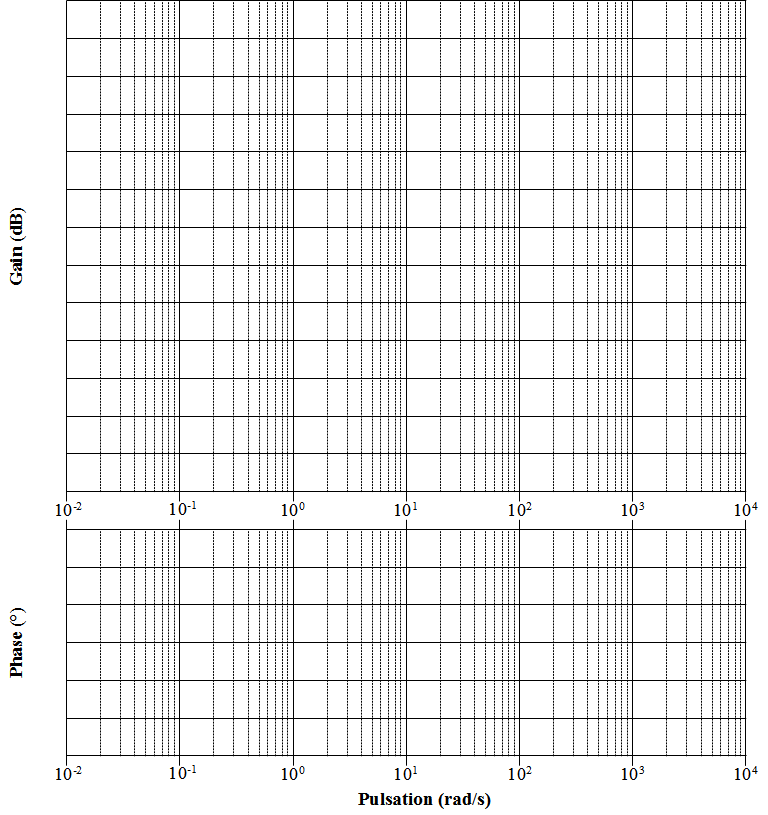
\includegraphics[width=\linewidth]{BodeVierge}
\end{center}

\subparagraph{}\textit{Tracer le diagramme de Bode de la fonction de transfert suivante : $F_2(p)=\dfrac{10}{\left(1+10p\right)\left(10+p\right)}$.}
\begin{center}
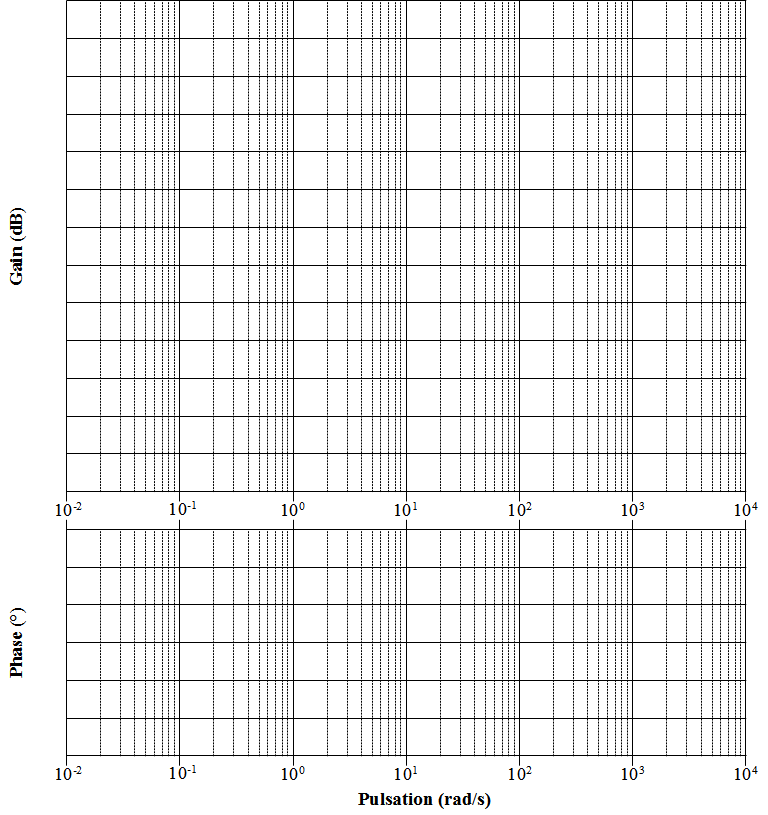
\includegraphics[width=\linewidth]{BodeVierge}
\end{center}

\subparagraph{}\textit{Tracer le diagramme de Bode de la fonction de transfert suivante : $F_3(p)=\dfrac{40}{p\left(1+300p\right)}$.}

\begin{center}
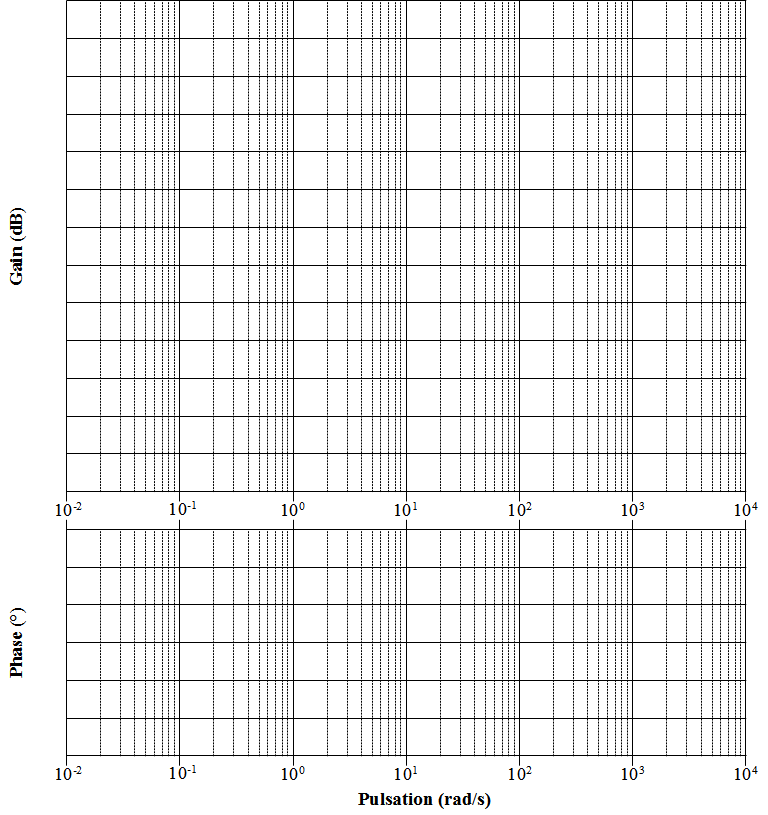
\includegraphics[width=\linewidth]{BodeVierge}
\end{center}